% \documentclass[rnd]{mas_proposal}
\documentclass[thesis]{mas_proposal}

\usepackage[utf8]{inputenc}
\usepackage{amsmath}
\usepackage{amsfonts}
\usepackage{amssymb}
\usepackage{graphicx}
\setcounter{secnumdepth}{4}
\usepackage{subfigure}

\title{Experience-Based Path Planning Framework for Real-time Learning from Demonstration}
\author{Natalia Leonila Quiroga Perez}
\supervisors{Prof. Dr. Paul G. Plöger\\
	Dr. Alex Mitrevski \\}
\date{July 2023}

\thirdpartylogo{images/migrave_logo_large.png}

\begin{document}

\maketitle

\pagestyle{plain}

\section{Introduction}

	This section presents a summary of the importance of robotic learning for therapy with children with Autism Spectrum Disorder (ASD), focusing on the needs of the therapist as the end user of the system. This is followed by a brief description of the approach, including its parts, the flow of the framework and a mathematical description.
	
	\subsection{Topic of This Master Thesis}

    Due to the growing acceptance of the use of robots in collaboration with humans in the same environment, Human-Robot Interaction (HRI) is being studied as a successfully emerging area. According to \cite{Sheridan2016}, there are four areas of application of HRI; namely, (i) human resources as supervisors in different areas where the tasks are repetitive but robots are still not independent (ii) robots that work in hazardous environments where humans do not have access, and whose movements are usually controlled remotely by an expert, (iii) autonomous robots, such as self-driven cars with humans as passengers, those navigate and plan by sensing their environment, and finally, (iv) robots in a social environment where they interact directly with people, teaching, entertaining, helping children and the elderly.
    
    Specifically, focusing on human-robot social interaction applications, robots used in therapy with children with ASD had a positive impact on the patients, as the children had certain preferences for the robot as a therapist instead of an adult; according to \cite{Prabha2019}, this is because children with this condition perceive the world differently and robots attract their attention.
    
    In order to encourage patients with autism to learn movements and body language during therapy, the typical procedure is human-human encounters; namely, a selection of imitation games are performed as described in \cite{Dautenhahn2004}, where the authors are aware that robots have limited movements, and this method would be difficult to use in a long term therapy, unless the robots increase their behavioural repertoire.
    
    Various procedures can be performed in order to increase the action libraries for the robots. From the naive approach of encoding each and every action, to the more sophisticated approach of using methods to collect demonstrations from humans include different types of motion capture such as kinesthetic guidance \cite{Kronander2013}, joystick control \cite{Jiang2013} and kinect camera\cite{Assad2020}. Collecting a large number of these demonstrations from non-experts to perform a motion learning procedure is not feasible and tedious for the demonstrator \cite{Chen2022}.
    
	\subsection{Relevance of robot learning for applications in therapy}
    
    During the study of robots in therapy for ASD, most of the time the main focus are the patients and how the robot affects their reaction, but the therapist also have a reaction to the involvement of robots. In the study by \cite{Kulikovskiy2021}, the therapists are the main focus and their preferences are explored, if they do not feel comfortable with the inclusion of new technology and they do not understand how to use it, it may be the case that they go back to traditional methods.
    
    Therapists, as part of the end-user group, should be able to operate the robots with little training and effort. During the experiments performed by \cite{Kulikovskiy2021}, with real therapists and the robot Pepper, the main observations were: (i) therapists prefer to teleoperate the robot with Virtual Reality (VR) than to manipulate the robot with a kinesthetic interface; (ii) the use of VR provides a treatment integrity of 83.7\%, which is comparably higher than the 52.9\% of the kinesthetic interface; (iii) therapists found it easier to adapt the therapy to the children's needs with the use of VR; and finally (iv) the workload of task preparation was higher with VR than with kinesthetic interface. 
       
    For instance, the aim is to simplify this process for the demonstrator by making it more user-friendly and faster. The human ability to learn by imitation, and social mirroring \cite{Byrne2005}, inspired Learning from Demonstration (LfD), which has now become an area of extensive research.
    
    In LfD it is necessary to collect examples of optimal sequences of actions or trajectories in order to reproduce similar behaviours \cite{Piot2017}. This can be achieved in two ways; on one hand, Imitation Learning (IL) is a type of supervised learning that consists of learning the mapping between states and actions \cite{Dinyari2020}. On the other hand, Inverse Reinforcement Learning (IRL) has no knowledge of the reward function and tries to learn from the expert's demonstrations \cite{Reddy2019}.
    
\section{Problem Statement}
    
    The problem identified in this study is the complexity of the systems that focus on learning from demonstration, namely, given the extra work involved in learning a new system, therapists prefer to stick to the traditional methods. We define a complete system as one that can perform learning in an efficient, fast and friendly way for the end user, in this case the therapist. Namely, the systems proposed in \cite{Hua2021, Koenemann2012} work with external equipment that can be complex to use for a non-expert, as well as the approach of \cite{Si2021, Assad2020, Kulikovskiy2021}, where the movements are teleoperated and the robots do not perform any kind of learning as such, meaning that the movements have to be repeated for each session.
    
    According to \cite{Lopes2005}, LfD has three main difficulties: (i) how to collect relevant information to perform a task; (ii) how to convert data valid for a human into another body, in this case a robot; and (iii) how to select the important parts of the demonstration. This thesis aims to address these issues by: (i) performing self- and workspace exploration to collect relevant information, (ii) transforming human skeleton-based data into robot embodiment positions by pose estimation, and finally (iii) selecting the significant demonstration path by learning from previous demonstrations.
    
    This thesis proposes an adaptable framework for autonomous self-mapping and learning from demonstration for robots by incorporating IL and IRL to learn not only actions from humans but also intentions in real time. For the development and experimentation QTrobot from LuxAI \cite{qtrobot_safety_manual}, NAO robot and Kinova Gen3 in its Freddy configuration, we considered both its physical and software features. For the whole LfD process, the first step is to identify the robot's workspace and the constraints of its configuration; then the human action recognition is performed, which can be done by using different methods. For this study, we use depth skeleton motions \cite{Chen2016}, where the teacher's position is calculated with respect to the camera coordinate system placed on the robot's head in the case of QTrobot. Finally, path planning and trajectory learning.
    
\section{Related Work}
    
    This section describes the state of the art for several areas of interest that will be part of the development of the project.
    
    \subsection{Autism Therapy}
    
    Patients with autism have problems with communication in general, as well as repetitive behaviours and restricted interests. During diagnosis, according to \cite{Brentani2013}, it is possible to identify the syndrome by noticing a lack of social interaction and affection with others, as well as repetitive body postures and lack of eye contact.  Depending on the level of autism, the treatment and synthoms may vary but in general the main focus is to increase their level of communication, this can be done by understanding non-verbally other people; namely understanding the tone of their voice, body posture, facial expressions and hand motions. As they tend to copy repetitive gestures \cite{Dautenhahn2004}, the therapy usually include repetition of movements that the patient has perform. These restricted and repetitive behaviours (RRBs) are implemented in an early age and tend to reduce as time goes by and the patients' cognitive ability increases \cite{Leekam2011}. ASD experts propose that the earlier the therapeutic intervention, the better the development of a normal adult life. Many treatments involve external assistance such as pets, computers, virtual reality, and robots, some of which have positive results compared to others, but also therapy may vary from patient to patient \cite{Scassellati2012}.
    
    \subsection{Learning from Demonstration}
    
    Robots are those designed to interact with humans. In most cases these robots have a humanoid shape or appearance, but the degrees of freedom (DOF) vary between them, some examples are Kaspar with 17 DOF\cite{Kaspar2023}, QTrobot with 12 DOF \cite{qtrobot_safety_manual}, Nao with 25 DOF \cite{softbankrobotics}, Pepper with 20 DOF \cite{softbankrobotics} and Zeno with 12 DOF \cite{Papakostas2021}. Given the large number of DOF they represent, programming them became a difficult task even for experts. Nevertheless, this difficulty leads to methods of autonomous learning; namely, learning by demonstration. This learning process tends to be natural and intuitive for the demonstrators, i.e. they should not be given long sets of technical instructions; demonstrations are safer for the robot than using a trial-and-error learning process, which can damage the robot and takes longer for each new learned movement \cite{Bandera2012}. Ideally, direct mapping can be performed, but the number of DOF become a problem, and direct mapping is not recommended in uncontrolled environments due to the possibility of collision with external agents or objects \cite{Bentivegna2004}.
    
    However, considering that human and robot bodies have similar general characteristics, a one-to-one mapping is possible in some cases. Nevertheless, it is important to contemplate the following strategies considering the DOF; one-to-many, many-to-one or many-to-many mapping \cite{Alissandrakis2007}. In all cases, it is necessary to have a clear understanding of what is the expected result of the mimicking and which strategy to follow; for example, the movement has to maintain certain angular configuration to avoid obstacles or the position of the end effector has to be maintained \cite{Bandera2010, Shin2001}.
    
    The imitation learning task is divided into two important parts: (i) the observation process, which involves data collection, and (ii) the imitation process, where the imitator can follow three strategies to imitate: the end-point level, where only the position and orientation of the end effector matter, the trajectory level, where velocity matters, and the path level, where spatial properties matter more than velocity \cite{Alissandrakis2002}.
    
    For the observation process, various approaches use external hardware such as touch sensors, cameras and external devices to accurately identify the target pose \cite{Hua2021}. Previous work such as \cite{Itauma2012, Liu2015} uses a Kinect sensor to track the human skeleton model to estimate the human pose, but the experiments are affected by sensor quality, light exposure and processing speed. Other approaches use a mobile phone to create the path for the robot, the device is moved as required and the robot follows the path. These experiments require a set of training data, and the results depend on the number of attempts made by the user; in particular, if there is one failed sample, the failure needs to be compensated for by many more correct samples \cite{Mandlekar2018}. In order to analyse the skeleton data, it is necessary to formalise a mathematical expression that optimises an imitation metric \cite{Billard2004}; this procedure can be done with the help of a geometric model such as Denavit-Hartenberg (DH) \cite{Fadli2018}. \cite{Assad2020} \cite{VanPerre2015}, which describes the relationship between successive joints and is used to place each of them in a given coordinate frame using a Homogeneous Transformation (HT) to calculate the relative position of each joint. Finally, some authors replace visual inputs with other types of data, such as markers, but these are often invasive and must be used in controlled environments to avoid disturbance; in particular, one of the common failures of this approach is its poor adaptability to natural environments \cite{Mohammad2009, Dillmann2004}.
    
    Of course, IL has disadvantages. Given that human movements are intended to be learned, it is challenging to apply this procedure to a non-humanoid robot. The ideal scenario would be to have a robot with a human-like shape and the same number of DOF moving in a similar way, but this is rarely the case \cite{Ravichandar2020}. Most applications using IL only consider the upper body, as shown in \cite{VanPerre2015}, due to the complex control system that requires the legs to move. Another important factor to mention is that these works do not take into account the speed of movement of the robot joints, which can cause damage to the structure. 
    
    \subsection{LfD in Therapy}
    
    In the context of therapy and rehabilitation, especially in the treatment of autism, showing a patient movements to imitate is a very efficient technique to learn movements or to associate them with an activity; in addition, this can also help to the patients to relate places with everyday movements. Therefore, they can perform independently certain activities, such as brushing their teeth, cleaning themselves and other basic needs. According to \cite{Cabibihan2013}, 6\% of robots that they mention are adaptable to the user's needs. The adaptability of the robot is important, not just because the environment where the interaction occurs, but more important, to modify and customize progressively the complexity of the therapy \cite{Dickstein2018}. The behavioural repertoire of the robot is usually limited. Programming new postures or sets of movements is a complicated task that requires a lot of time, effort and knowledge in the field of robot programming and control.
    
    Imitation learning in robotics has many advantages for the end user. As there is no need to create programmes for each task or action, no technical knowledge is required, complex postures can be achieved and the learning effort can be reduced. More specifically, in this application we focus directly on the needs of the therapist \cite{Ravichandar2020, Kulikovskiy2021} and indirectly on the needs of the patient. 	
    
    \subsection{One-shot Learning}
    
    One-shot learning attempts to learn the action after each demonstration without prior training \cite{Yan2010}; for example, this type of technique can overcome the problem of insufficient samples while still producing an expected result. A skeleton-based method for dynamic hand gesture recognition using a reinforcement learning network (GREN) based on one-shot learning is proposed in \cite{Chunyong2020}, where only a small subset of gestures from a dataset was taken as training samples; in an evaluation experiment, given 14 classes, the final accuracy achieved was 82.29\%, and even higher accuracy with the GREN network in a 28-class recognition setting, but the learning process is still done in a semi-supervised manner by training an encoder with metric learning techniques \cite{Sabater2021}. A limitation of one-shot learning methods is that robots cannot imitate actions with good precision and accuracy with a single sample, and either learn progressively by try-and-error.
    
    \subsection{Gaussian Mixture Model}
    
    A Gaussian Mixture Model (GMM) is a probabilistic model that represents a probability distribution represented as a mixture of multiple Gaussian distributions. Usually, it is used as a parametric model that takes data as continuous measurements, and assumes that it comes from a combination of several Gaussian distributions. GMM parameters are estimated during the iterative Expectation-Maximization (EM) over the training data. One of the advantages of GMM is its ability to create smooth approximations \cite{Reynolds2009}, in our case trajectories. GMM is commonly used in the context of one-shot learning and imitation learning, uses generalised parameters which weights are associated with the Gaussian parameters that allows direct interaction with users. Among the methods capable of imitating movements, a decision-based rule approach is used in \cite{Itauma2012} with 96\% accuracy and a linear regression normal equation with 72\% accuracy. In \cite{Wu2020}, GMMs are used as part of a framework for autonomous impedance regulation, where the robot uses IL to learn the geometry of a task; namely, opening a door. For this purpose, they used GMM and Gaussian Mixture Regression (GMR) to encode the trajectory offline and reproduce it online. The results show that the trajectory's geometry and the GMM generated parameters were always synchronized. On the other hand, a disadvantage is that for every new task, many demonstrations must be performed and the training has to be updated as well.
    
    \subsection{Reinforcement Learning}
    
    Reinforcement learning (RL) is a machine learning (ML) technique in which an agent learns a behaviour through trial and error, in which the agent interacts with its environment, and its goal is to maximise the rewards it receives. RL generally assumes that the learning problem can be modeled as a Markov Decision Problem (MDP). An MDP defines a sequence of decisions to be made by the agent. These actions, product of the decision process, influence the immediate reward and subsequent actions, called states, through future rewards \cite{Kaelbling1996, Brunke2022, Elguea2023}. In \cite{Elguea2023} the MDP is represented as a tuple shown in \ref{eq:tuple_RL}. 
    
    \begin{equation}
    [S, A, P(s'|s, a), R(s, s', a), \gamma]
    \label{eq:tuple_RL}
    \end{equation}
    
    Where $S$ is the set of possible states that the agent can take, $A$ is the set of actions that the agent can make, $P(s'|s, a)$ is the probability of transition from a state $s$ to a future state $s'$ through the action $a$, $R(s, s', a)$ is the reward expected from moving from $s$ to $s'$ and it is calculated through the reward function, and $\gamma$ is a discount factor that affects to the reward function. A policy $\pi(a|s)$ is the mapping states and the probabilities of the actions, i.e. the total amount of reward the agent expects to receive if the goal is reached. Thereafter, $\pi(a|s)^*$ is defined as the optimal policy \cite{Hussein2018, Elguea2023}. 
    
    One of the applications of RL is shown in \cite{Kober2010}, where it is used for learning human movements efficiently by imitating a trainer within two experiments with a real robot with 7 DOF, the system uses RL for self-improvement, namely its adaptation is an expectation-maximisation algorithm whose return is $0.937$, higher than the return of finite difference gradients (FDGs) and vanilla policy gradients (VPGs), which was 0.907 in both cases. In the application of \cite{Fuernkranz2012}, RL was used as part of a preference-based learning framework where the reward is not numerical but qualitative. 
    
    RL requires a large number of samples and trials to complete the learning process, which generally makes it difficult to use for robot manipulation \cite{Hua2021}. On the other hand, different methods are also used to find optimal paths, such as Evolutionary Algorithms (EAs), which can be used to find motor trajectories for low and high numbers of DOFs \cite{Nolfi2000}; similarly, Particle Swarm Optimisation (PSO) \cite{Zhang2015} and Ant Colony Optimisation (ACO) \cite{Zhang2010} try to simulate the movements of living creatures to generate paths.
    
    \subsection{Inverse Reinforcement Learning}
    
    Inverse Reinforcement Learning (IRL) is an ML technique that solves the inverse problem of RL as the name indicates. IRL aims to model the observed behaviour of an external agent. It models the behaviour as an MDP, but whereas RL tries to learn a policy $\pi$ that maximises reward, IRL takes a set of behaviours $\mathcal{B}$ or trajectories and assumes they belong to a policy $\pi^\mathcal{B}$, then learns a reward function from samples of the mentioned policy \cite{Heim2019}. Namely, IRL deals with the problem of finding a reward function when a policy or set of demonstrations are available, it is a key method to implement IfD \cite{Arora2021}. The problem with this procedure is that more than one reward functions can represent the set of trajectories \cite{Russell2000}. 
    
    IRL is used in HRI for several applications, as part those, it has been used in real-world applications; as part of those, self-driving cars, where the agent learns from demostrations the desired behaviour while dealing with many variables such as speed, distance, signs and pedestrians \cite{Arora2021} . Another application of IRL is shown in \cite{Kretzschmar2016}, where the goal was learning navigation in a enviroment with static obstacles and pedestrians from human walking trajectories. Another application is presented in \cite{Chen2023}, where the authors present a transition framework from IRL to RL, where a robot interacts with humans by acting as a mall receptionist and encourages visitors to use hand sanitiser. 
    
    Real world data is usually expensive and IRL has the advantage of working in tasks with limited access to data collection as shown in \cite{Chen2023}. The agent can learn preferences or trajectories from high-dimensional human demonstrations. In the work of \cite{Bhattacharyya2020}, they use an IRL framework to learn human intentions; IRL has been shown to outperform RL for learning everyday activities such as preparing cereal, where the reward function is difficult to identify. 
    
    The agent can learn preferences or trajectories from high-dimensional human demonstrations. In \cite{Bhattacharyya2020}'s work, they use an IRL framework to learn human intentions; IRL has been shown to outperform RL for learning everyday activities such as preparing cereal, where the reward function is difficult to identify. On the other hand, \cite{Hussein2019} use IRL in a medical application, namely their robot imitates a demonstrator to learn how to take on the role of a therapist, specifically to teach skills to children.  
    
    \subsection{Path Planning}
    
    Route planning is the process of determining a path to reach a destination on a map in the most efficient way possible. During the execution of the plan, the robot might encounter obstacles, but ideally still reach the goal. As the number of DOF of the manipulator increases, the solution of the problem becomes more complex, for example, the free space has to be constructed in order to solve the problem \cite{Siegwart2011}. 
    
    Real-time path planning is used in many applications, some of which are obstacle avoidance for self-driving cars \cite{Chaocheng2015} and pouring liquids \cite{Yamaguchi2015}, which have in common that the goal is dynamic, namely it keeps changing during execution or planning. According to \cite{Xie2020}, IL and IRL are both used for path planning based on LfD, namely IL works with path planning in free space and considering obstacle avoidance; on the other hand, IRL helps to train real-time trajectories and adjust the planning. 
    
    As mentioned earlier, planning is more complex with more robots, in the case of humanoid robots they usually have two arms that need to coordinate with each other to avoid collisions and work together. In \cite{Pecora2018}, for two collaborating robots, the authors consider certain constraints for the planning, the paths are time-dependent, and in case of a critical position, they perform a following procedure, namely one moves after the other.
    
    Humanoid robots also have similar systems for trajectory planning as in the case of \cite{Kuffner2001} with the robot H6; in their case, the geometric model of the environment is known as well as the initial and goal positions. The computational average time in seconds to perform the tasks over 25 trials that were evaluated are: (i) reaching under a chair in 324s, (ii) lifting a leg over a box in 48s, and (iii) reaching over a table in 371s. Rapidly-exploring Random Trees (RRTs) were used for panning. RRTs can be used to speed up the planning time in an algorithm; each node of the trees is generated by random sampling \cite{Veras2019}.
    
    As part of the planning, some frameworks have been developed with optimal characteristics. $Lightning$ is a framework proposed by \cite{Berenson2012} shown in Fig. \ref{fig:lightning_framework}, for high-dimensional spaces. $Lightning$ has two main parts running in parallel: (i) a Retrieve Repair (RR) for learning from previous experience stored in a library, and (ii) Planning from Scratch (PFS) for new trajectories. As part of the RR they used bidirectional RRTs (BiRRTs). Their experiments were performed on the PR2 and a surgical robot, both simulations; they show that the RR module outperforms PFS in over 90\% of the tests.
    
    Another framework developed by \cite{Coleman2015} is called $Thunder$ shown in Fig. \ref{fig:thunder_framework}, it is capable of solving high dimensional planning problems and is compared to $Lightning$, the main differences are that $Thunder$ uses Sparse Roadmap Spanner (SPARS) to store experiences, Nearest Neighbours (NNs) and A* search in the RR. The experiments tested on a humanoid robot called HRP2 showed that $Thunder$ uses 98.8\% less memory than $Lightning$ and the average path planning times in a static environment are 0.88s and 2.61s and in a dynamic environment 0.85s and 8.59s for $Thunder$ and $Lightning$ respectively.
    
    \begin{figure}[h]
    	\centering
    	\subfigure[Overview of $lightning$ Framework \break (taken from \cite{Berenson2012})]{\label{fig:lightning_framework}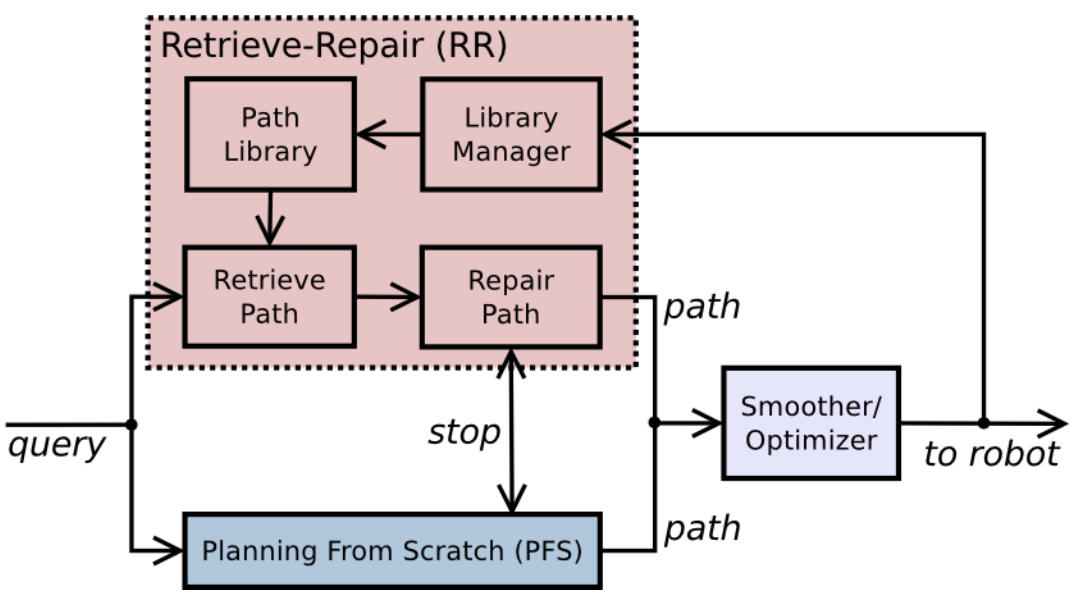
\includegraphics[width=0.45\textwidth]{images/lightning_framework.png}}
    	\subfigure[Overview of $Thunder$ Framework \break (taken from \cite{Coleman2015})]{\label{fig:thunder_framework}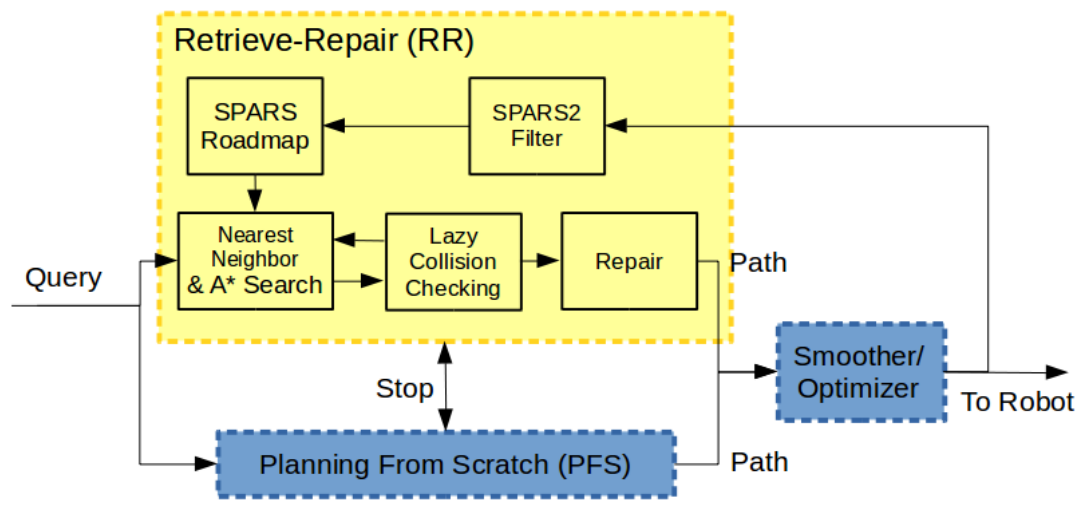
\includegraphics[width=0.45\textwidth]{images/thunder_framework.png}}
    	\label{fig:related_frameworks}
    	\caption{Comparison of path planning frameworks}
    \end{figure}   
    
    \subsubsection{Graph Search}
    
    In order to represent the robot's workspace, graph construction is used as an off-line solution to gain knowledge of the free space in advance, saving computational time when performing a demonstration and being able to do it in real time \cite{Siegwart2011}. 
    
    Graphs are widely used in path planning to provide a discrete representation of space and its connectivity. \cite{Phillips2012} use an experience graph (E-graph) to speed up the planning process. They are able to use parts of previous paths to speed up the procedure, in the results they show that the procedure is significantly faster than Weighted A*, Probabilistic Roadmap (PRM) and Randomised Planner (SBL); but not than Bi-directional (RRTs). In the \cite{Cohen2012} approach, they used a two-armed robot to work collaboratively; its workspace was described as a graph $G = (S, E)$, with states $S$ and edges $E$, where a state $s$ is defined as $(x, y, z, \theta_{yaw}, \theta_{1}, \theta_{2})$ to describe the position of the end effector, the orientation of the object, and the two joint angles respectively. For the search, they used Anytime Repairing A* (ARA*), which is faster than A* in their experiment results.
    
    On the application of \cite{Natarajan2023}, using the Kinova Gen3 arm; they proposed a graph search with incremental path optimisations for high-dimensional spaces, where the heuristic is the Eucledean distances between two nodes in the joint configuration. They used Weighted A* to perform the search and compared it with BiRRTs.
    
    \subsubsection{Path Smoothing}
    
    Another part of path planning that comes at the end, independent of the search procedure, is smoothing, which is performed as a final step and makes the trajectories more suitable for reproduction on a real robot or simulation as shown in \cite{Berenson2012, Coleman2015}; where $Lightning$ uses path shortening when the trajectories are not straight. Smoothing is part of noise reduction and can be performed linearly, such as Meadian and low-pass filters, and non-linearly \cite{Siegwart2011, Ravichandar2020, Si2021}.
    
    There are different types of smoothing that have different goals, such as creating smooth curvatures, preserving continuity, or shortening paths. As shown in \cite{Ravankar2018}, some methods are interpolation, path smoothing with special curves such as Dublin's curve or clothoid.
    
    \subsection{Self-Collision Avoidance}
    
    When it comes to robots with different amounts of DOF, or with a structure such as a human body, it is important to take care of collisions so as not to damage the robot. In the case of \cite{Dietrich2012, Santis2007}, a non-collision system is designed for a humanoid robot with two arms; this module is based on artificial repulsive potential fields, where each joint has a potential value depending on the distance to other joints, to cause a repulsive effect between elements of the same robot and thus avoid collisions. Another method used is the creation of volumes to simulate the body of the robot, in the case of \cite{Stasse2008}, a series of spheres and toruses are used to simulate what they call Sphere-Torus-Patches Bounding Volume (STP-BV); the main objective of this reconstruction is to maintain continuity in the volume gradient and to reconstruct it as accurately as possible. This procedure goes hand in hand with a control system of the collision avoidance module, therefore real-time execution is compromised. Although these are the most common methods, there are also simulations such as the work presented in \cite{Fang2015}, which is a self-collision avoidance system for humanoid robots; in this case, the Support Vector Machine (SVM) is used in conjunction with quadratic Lagrangian interpolation to estimate the positions of all the joints of the robot; it should be noted that this work has not been implemented in a real robot, but it showed efficient results in the experimental simulation.
    
    \subsection{Robot Kinematics}
    
    Robot kinematics can be divided into two major categories, namely Forward Kinematics (FK) and Inverse Kinematics (IK). FK uses equations to find the position and orientation of a joint given the joint angles, usually the end effector. An application of FK in IL is to control the human pose, namely it reconstructs the 3D pose of a target with respect to all joints and establishing the relationship between the $k-th$ joint with respect to its parent joint \cite{Li2021}. While IK is used to find the joint angle variables that satisfy a desired pose of the robot during its manipulation \cite{Hayat2015}. Namely, IK is used to control the position of a robot. An application of IK in IL is to re-estimate poses whenever collision is performed.
    
    \subsubsection{Forward Kinematics}
    
    Forward Kinematics is used to represent the position and orientation of the manipulator's end effector. \cite{Assad2020} used FK to mimic arm movements, namely it is a computational tool based on the chain rule for spatial transformations with respect to the base frame. In the work of \cite{Malik2017}, the hand position of a user is estimated with a hybrid FK system; where all poses are derived from the initial hand position, the aim is to detect finger positions for signal recognition. FK is often used to estimate the position of the human-based skeleton, in \cite{Huang2022} the model uses Denavit-Hartenberg (DH) to eliminate the ambiguous solutions for the angles and non-continuous movements. One of the advantages of FK is that the number DOF of the robot does not significantly affect the computational time, the solution is calculated straightforward. In the work of \cite{Shao2015}, an FK simulator is developed for a 6 DOF surgical robot, with the aim of predicting the robot's behaviour and improving its performance during surgery on patients.
    
    \subsubsection{Inverse Kinematics}
    
    Inverse Kinematics determines all possible configurations of angles for a chain of links. IK can be a geometry-based calculation for a given position and orientation of the end effector with respect to the base frame. In contrast to FK, this method results in several solutions from which the most suitable one must be selected according to the requirements of the system \cite{Mueller2019}. This method is used by \cite{Koenemann2012, Koenemann2014} to maintain the balance of an NAO robot when making imitations; for this, the center of mass must be within the support polygon at the robot's feet. In the discussion presented in \cite{Martin2003}, different methods for solving the IK for skeleton manipulation in real time are proposed and compared in real applications to find the best method in terms of speed and accuracy. According to this comparison, the Jacobian method cannot be used in real time due to the complexity of the mathematical calculations; therefore, the algebraic method and the Cyclic Coordinate Descent (CCD) method are proposed. For the imitation process, other authors use the chain model, which consists of a biologically inspired model of the mirror neuron system that controls the motors to direct them towards a target \cite{Chersi2012}. In the proposal of \cite{Rokbani2014}, a system called Firefly Algorithm (IK-FA) is proposed, with which the position of the joints of a robot with 2 and 3 limbs can be calculated in order to maintain a target position of the end effector.
    
\section{Limitation and Deficits in the State of the Art}
    
    In the current work of the LfD, robotic actions that are used in therapy or rehabilitation are usually pre-programmed offline, teleoperated actions, or are obtained through a kinesthetic interface. On the other hand, those systems require large sets of training data that is expensive to collect \cite{Dinyari2020, Yan2010, Mandlekar2018}. We aim to create a friendly end-user framework that reduces the therapist's workload and requires fewer demonstrations to perform movement imitation.
    
    In this particular application, different types of robots will be used. Due to the differences between them and the clear difference with human embodiment and kinematics \cite{Koenemann2012}; it becomes a challenge to generalise the learning of human movements with direct mapping, even with computer vision methods where data processing algorithms are required for learning, replication and storage \cite{Liu2015}, so that performing actions through movements requires processing of the stored data by a learning algorithm \cite{Kober2010}. In some cases, the types of actuators used on a robot limit the movement of the joints; therefore, not all positions can be achieved and learned \cite{Almalki2020}.When using a new robot platform with a different morphology and workspace, it is necessary to implement new joint trajectories to achieve the desired postures \cite{VanPerre2015}. Thus, the proposed framework aims to work with different robots under basic tuning and simple pre-exploration to get some basic knowledge of the environment. 
    
    The imitation movements are only of the upper limbs, because the therapists were afraid that the children would imitate the walking style of the robot. This includes some constraints in the coordination of the arms of the robots, which are not specified or taken into account in the work of \cite{Liu2015, Fadli2018, Suleiman2008}. In the work of \cite{VanPerre2015}, some constraints were considered to perform imitation in three different robots but those were simulated and only limited movements.
    
    Some frameworks, as is the case of \cite{Berenson2012, Coleman2015}, optimise the path planning for learning new motions by correcting previous trajectories, and got very optimistic results with little data in their library, unfortunately these algorithms showed results only in a simulation of a single robot and were not proven in a real robot in the real world. 
    
\section{Learning from Demonstration approach}

    The aim of this project is to create a framework that facilitates the process of learning upper limb body movements to extend the action repertoire of robots by capturing skeletal data from non-expert users using an external RGB-D camera. Subsequently, this library will be stored gradually with new actions in order to use them in therapy with ASD patients.
    
    The functionality of the framework is divided into two phases, one of which is carried out only once before the non-expert starts the demonstrations; namely, the robot has to carry out a discretization of the environment. And the second phase is the action learning process as such. An overview of both phases is shown in the figure \ref{fig:framework_overview} for better understanding.
    
    
    \begin{figure}[h!]
    	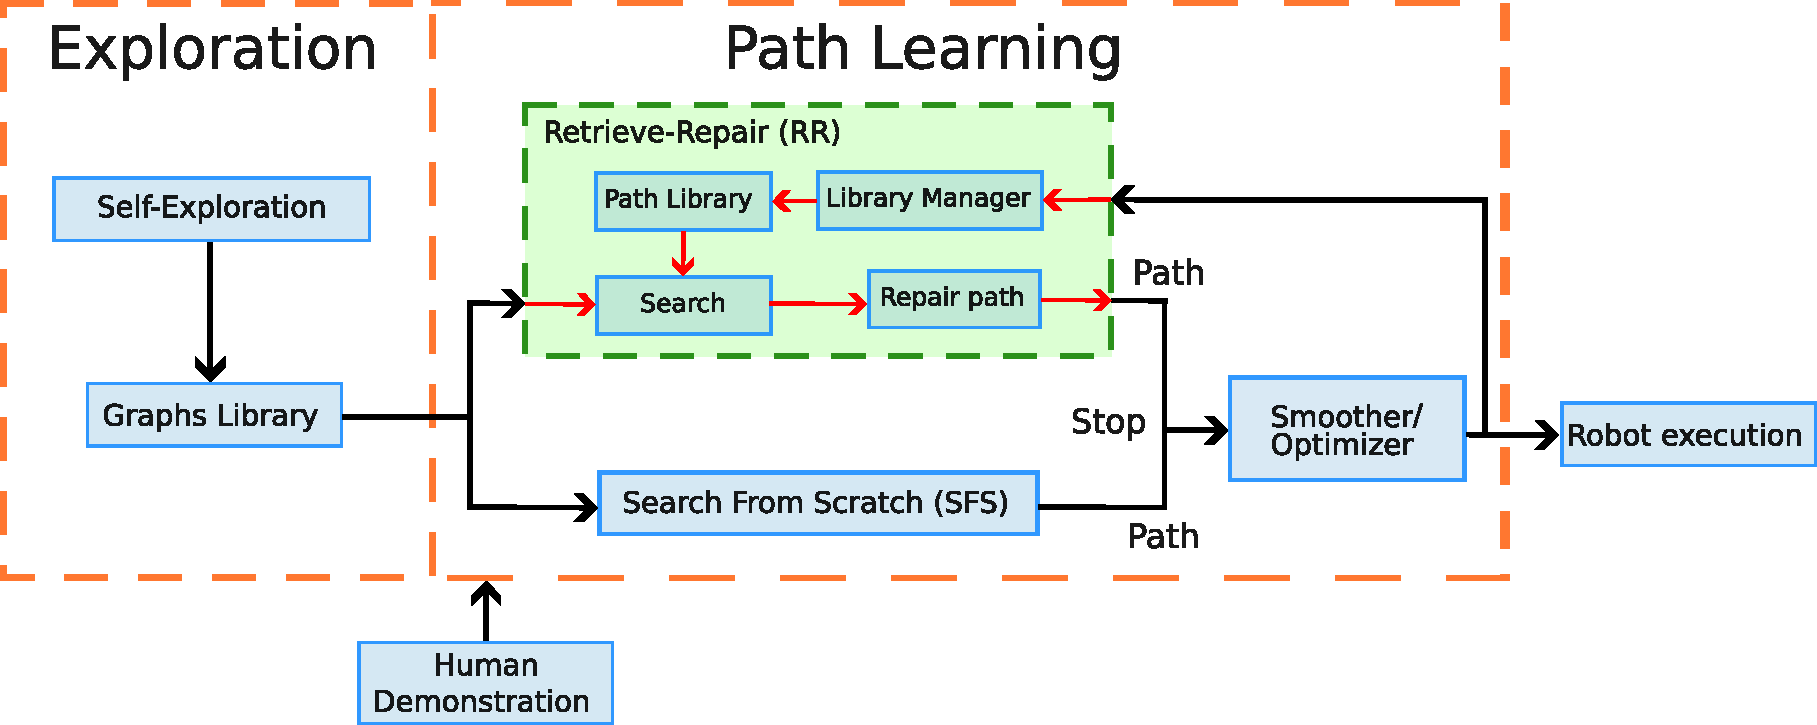
\includegraphics[width=\textwidth]{images/framework_overview.pdf}
    	\caption{Learning from demonstration framework overview}
    	\label{fig:framework_overview}
    \end{figure}
    

\subsection{World Exploration}
    
    By performing a space exploration within the limits of the actuators in order to map and recognise the environment and possible obstacles present in its workspace, including its own body structure. The result of this exploration is a set of $2n$ graphs, where $n$ is the number of joints of one arm of the robot, namely, each joint has its own graph but all of them are connected given the joint dependencies of the manipulator. Each joint $j$ has a graph $G_j$ has a dependency on the graph $G_{j-1}$ of the previous joint $j-1$. 
    
    Let's consider just one arm of the robot. Then we can define a joint $j \in {1,2,..,n}$, for instance, the nodes and edges for its respective graph $G_j$ are described as follows:
    
	\begin{itemize}
		
		\item \textbf{Nodes:} The vertices or nodes of the graph $G_j$ represent reachable points for the joint $j$ in the Cartesian space and it stores the following elements: its position $(x, y, z)$, the angular positions of all previous joints $(1,2,..,j)$ as $(\theta_1, \theta_2,..,\theta_j)$, a state of free or occupied $(0, 1)$, and a list of $k$ joints that can reach the same spatial position in some configuration, it means that this position exists in at least one other graph. 	
		
		\item \textbf{Edges:} The links or edges of the graph $G_j$ is the Euclidean distance $d$ between two nodes that belong to the same graph. The value of $d$ is constant and determines the quality of the workspace; namely, the smaller the value of $d$, the higher the quality of the graph, which means the quality of the movements, the search time and the memory storage also increase; if the value of $d$ is larger, the memory storage and the search time are smaller, but the quality of the path is compromised. Therefore, $d$ has to be carefully tuned to a value that does not compromise either the movements or the time and memory costs. The value of $d$ is the same for all graphs $2n$.
		
	\end{itemize}  
  
   	\subsection{Skeleton representation}
   		The skeleton-based data stores the position of the human embodiment defined as $S^H$. Considering the skeleton upper body part, the joint called ``collar" is placed in the center of the body on the chest; this is for the human the base frame $B^H = (0, 0, 0)$, continuously, we can calculate the Spherical coordinates for all the human joints following the equations \ref{eq:radial_distance}, \ref{eq:polar_angle} and \ref{eq:azimuthal_angle}.
   	
	   	\begin{equation}
	   	r = \sqrt{x^2 + y^2 + z^2}
	   	\label{eq:radial_distance}
	   	\end{equation}
	   	\begin{equation}
	   	\theta = \arctan \frac{y}{x}
	   	\label{eq:polar_angle}
	   	\end{equation}
	   	\begin{equation}
	   	\phi = \arctan \frac{\sqrt{x^2 + y^2}}{z}
	   	\label{eq:azimuthal_angle}
	   	\end{equation}
	   	
	   	The transformation gives the polar angle and the azimuthal angle which are the direction of all links. These are then used to calculate the Cartesian coordinates of the robot on its own embodiment following the equations \ref{eq:x_cartesian}, \ref{eq:y_cartesian} and \ref{eq:z_cartesian}. 
   	
	   	\begin{equation}
	   	x = r \sin \phi \cos \theta
	   	\label{eq:x_cartesian}
	   	\end{equation}
	   	\begin{equation}
	   	y = r \sin \phi \sin \theta
	   	\label{eq:y_cartesian}
	   	\end{equation}
	   	\begin{equation}
	   	z = r \cos \phi
	   	\label{eq:z_cartesian}
	   	\end{equation}
	   	
	   	Once the desired pose of the robot is found, i.e. the coordinates $(x,y,z)$ of all the joints in Cartesian space, it is possible to search for these coordinates for each joint on its corresponding graph. This would lead to a specific angular configuration for all captured frames. Given the characteristics of the RealSense Depth Camera used, namely its frame rate for RGB of up to 30 fps \cite{realsense_manual} which means that the procedure must match that speed of calculation. 
   	
   	\subsection{Path Learning}
   	
	The second phase of the framework assumes that the space is partially known for the robot, due to the fact that not all reachable points of the workspace may be explored or there may be more than one robot configuration to reach that point, but enough points have been collected to avoid self-collisions and to detect the static obstacles as shown in the Fig. \ref{fig:mapped_graph}. A 2D example of the path planning learning is shown in the Fig. \ref{fig:path_planning_on_graph}. 
	
%	\paragraph{Real-Time Path Planning}\mbox{} \\ [10pt]
	\begin{figure}[h]
		\centering
		\subfigure[Initial graph]{\label{fig:mapped_graph}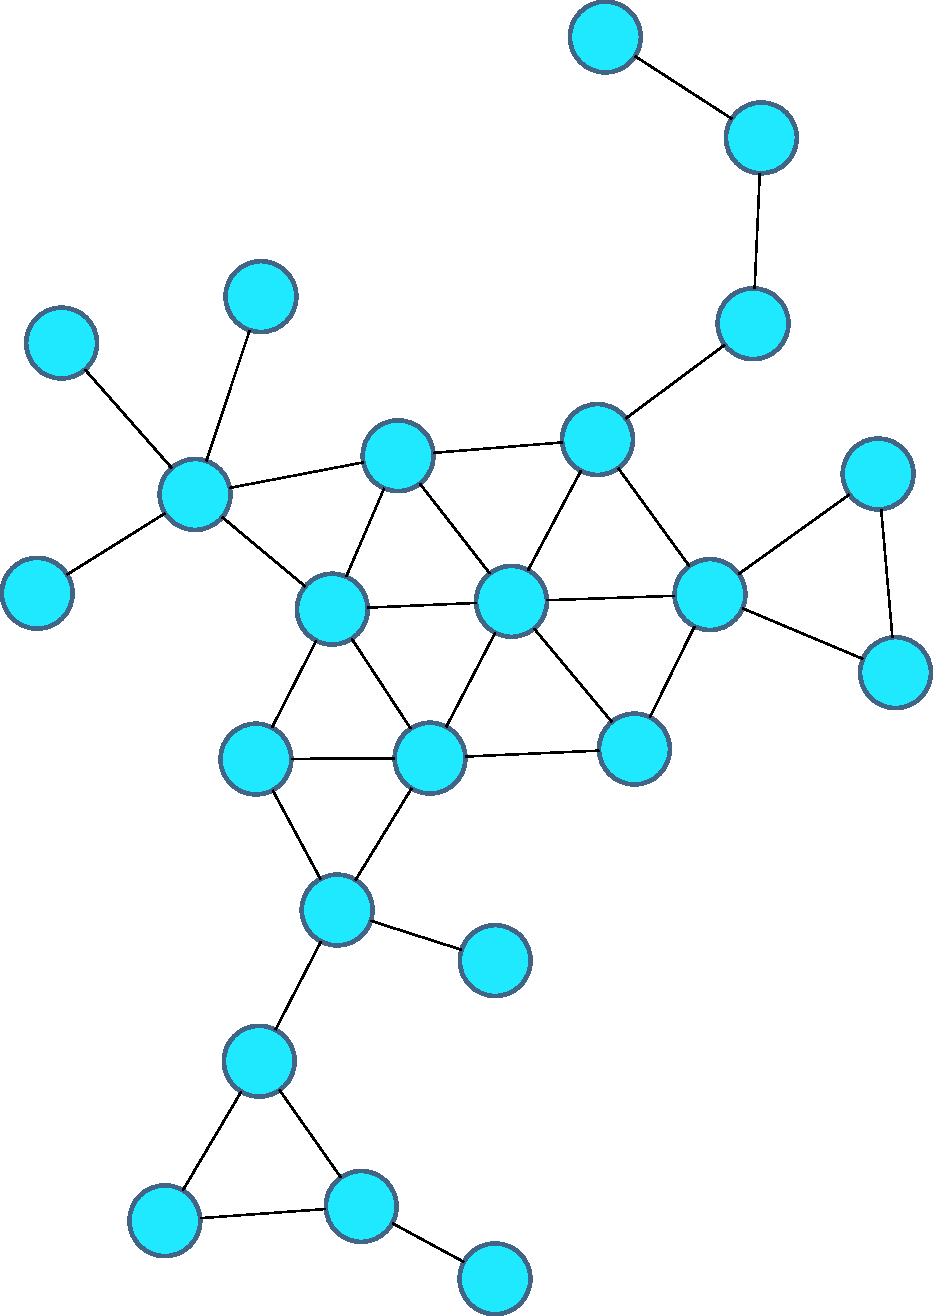
\includegraphics[width=30mm]{images/mapped_graph.pdf}}
		\subfigure[Trajectory from demostration]{\label{fig:trajectory}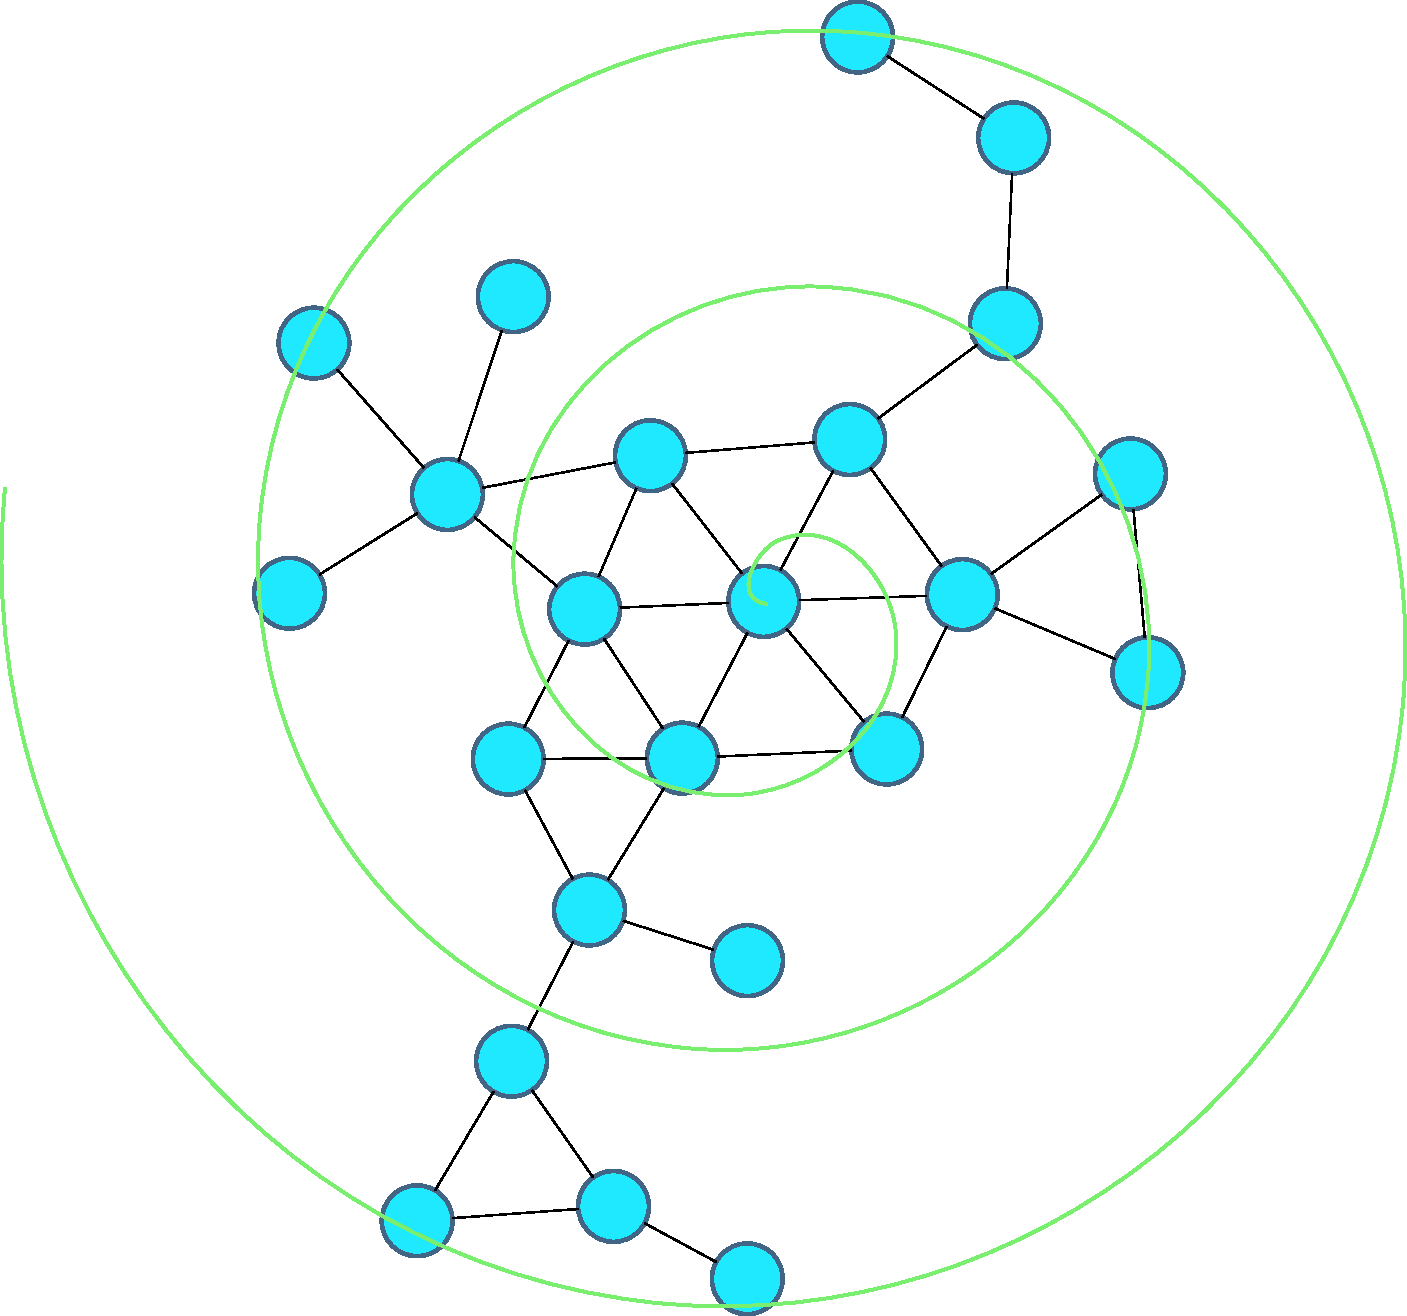
\includegraphics[width=45mm]{images/trajectory.pdf}}
		\subfigure{\label{fig:legend_graph}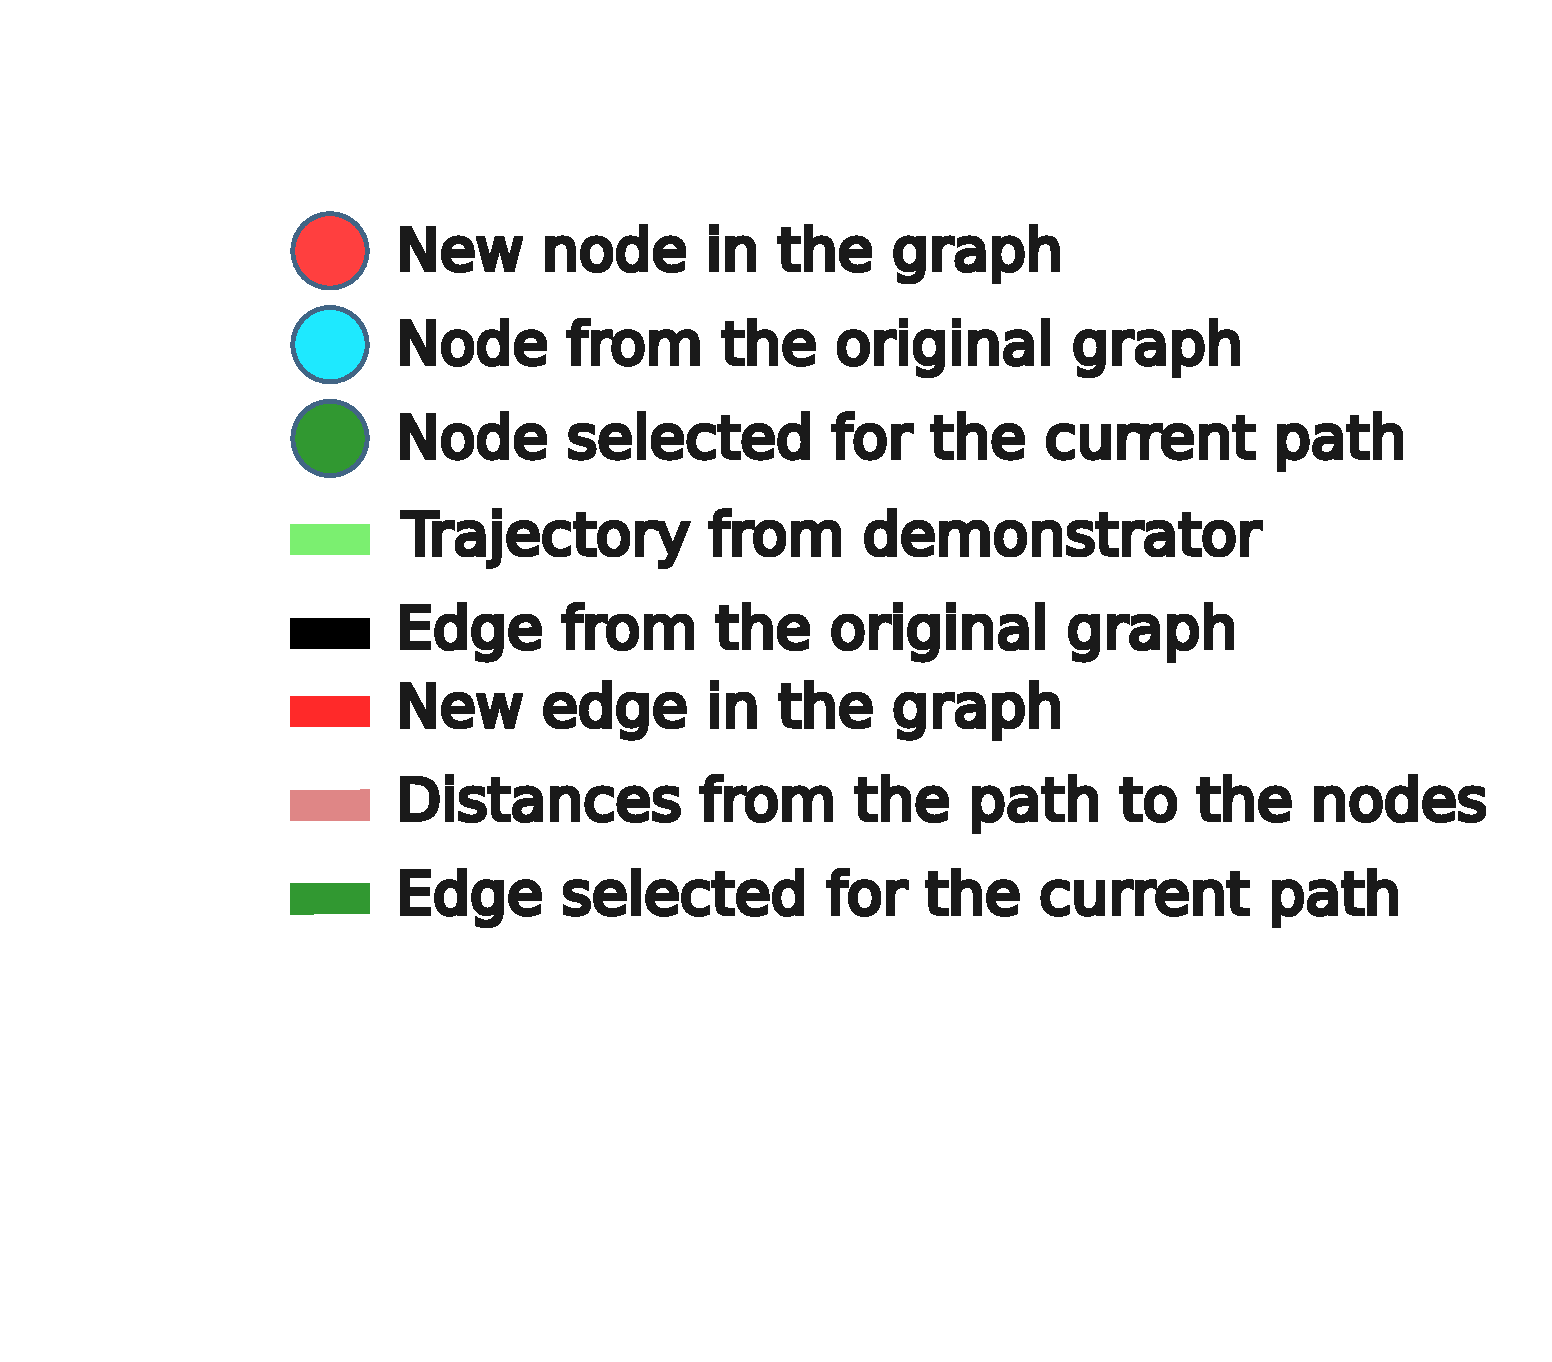
\includegraphics[width=55mm]{images/legend_graph.pdf}}
		\subfigure[Distance from the trajectory to the graph]{\label{fig:distances_to_trajectory}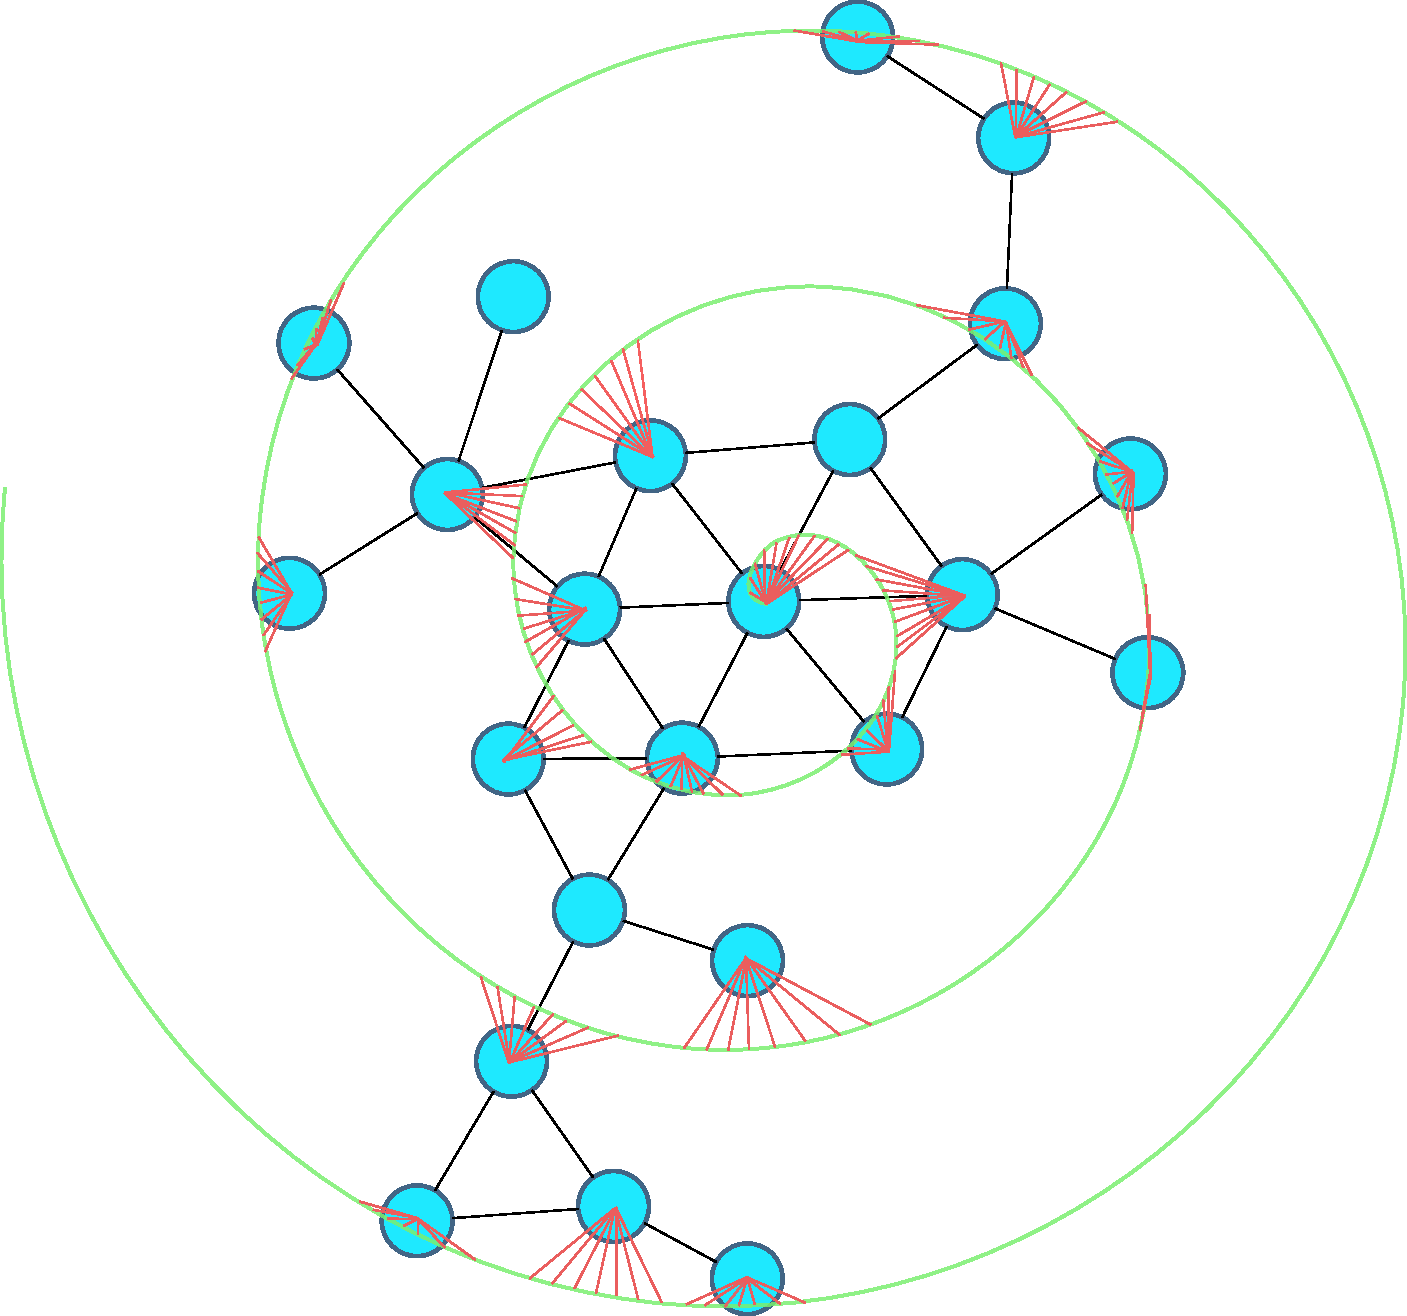
\includegraphics[width=45mm]{images/distances_to_trajectory.pdf}}
		\subfigure[New nodes added to complete the trajectory]{\label{fig:new_nodes_edges}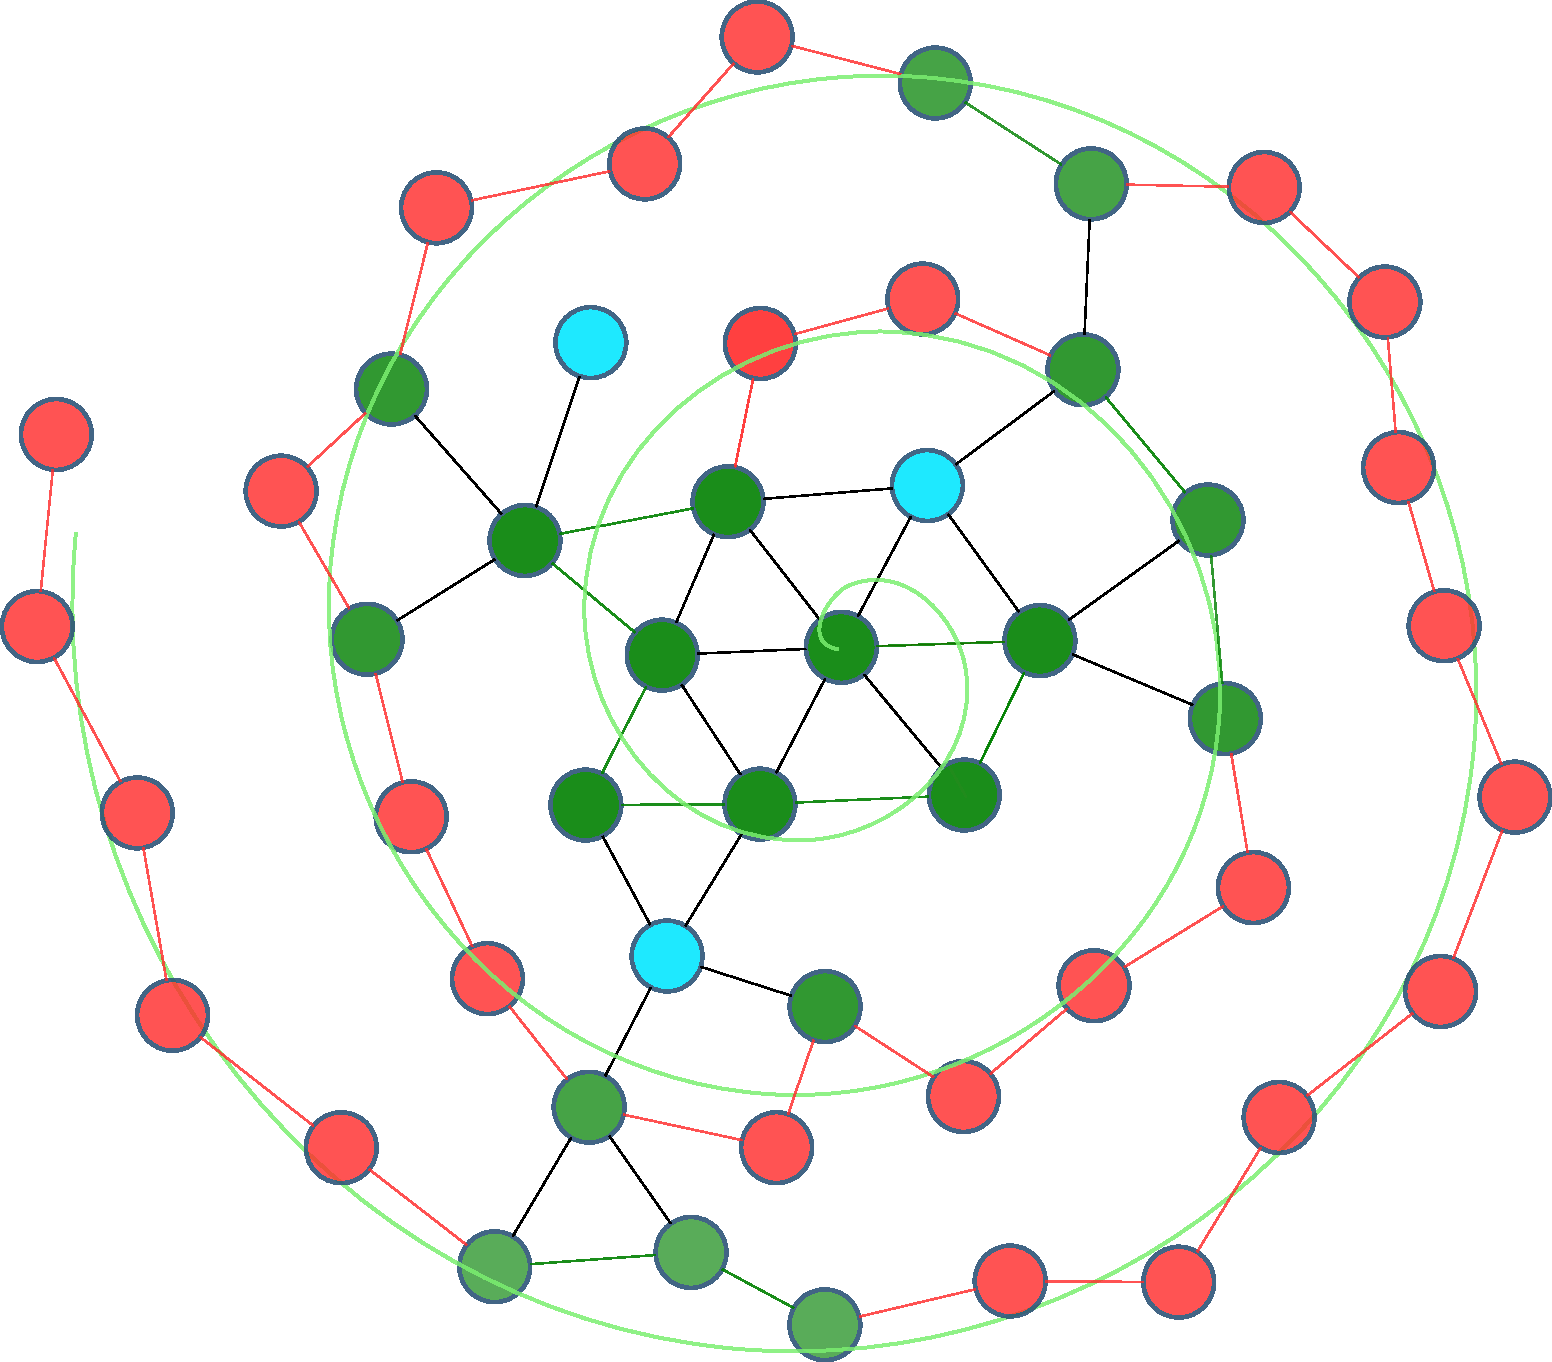
\includegraphics[width=45mm]{images/new_nodes_edges.pdf}}
		\subfigure[Path before smoothing]{\label{fig:node_trajectory}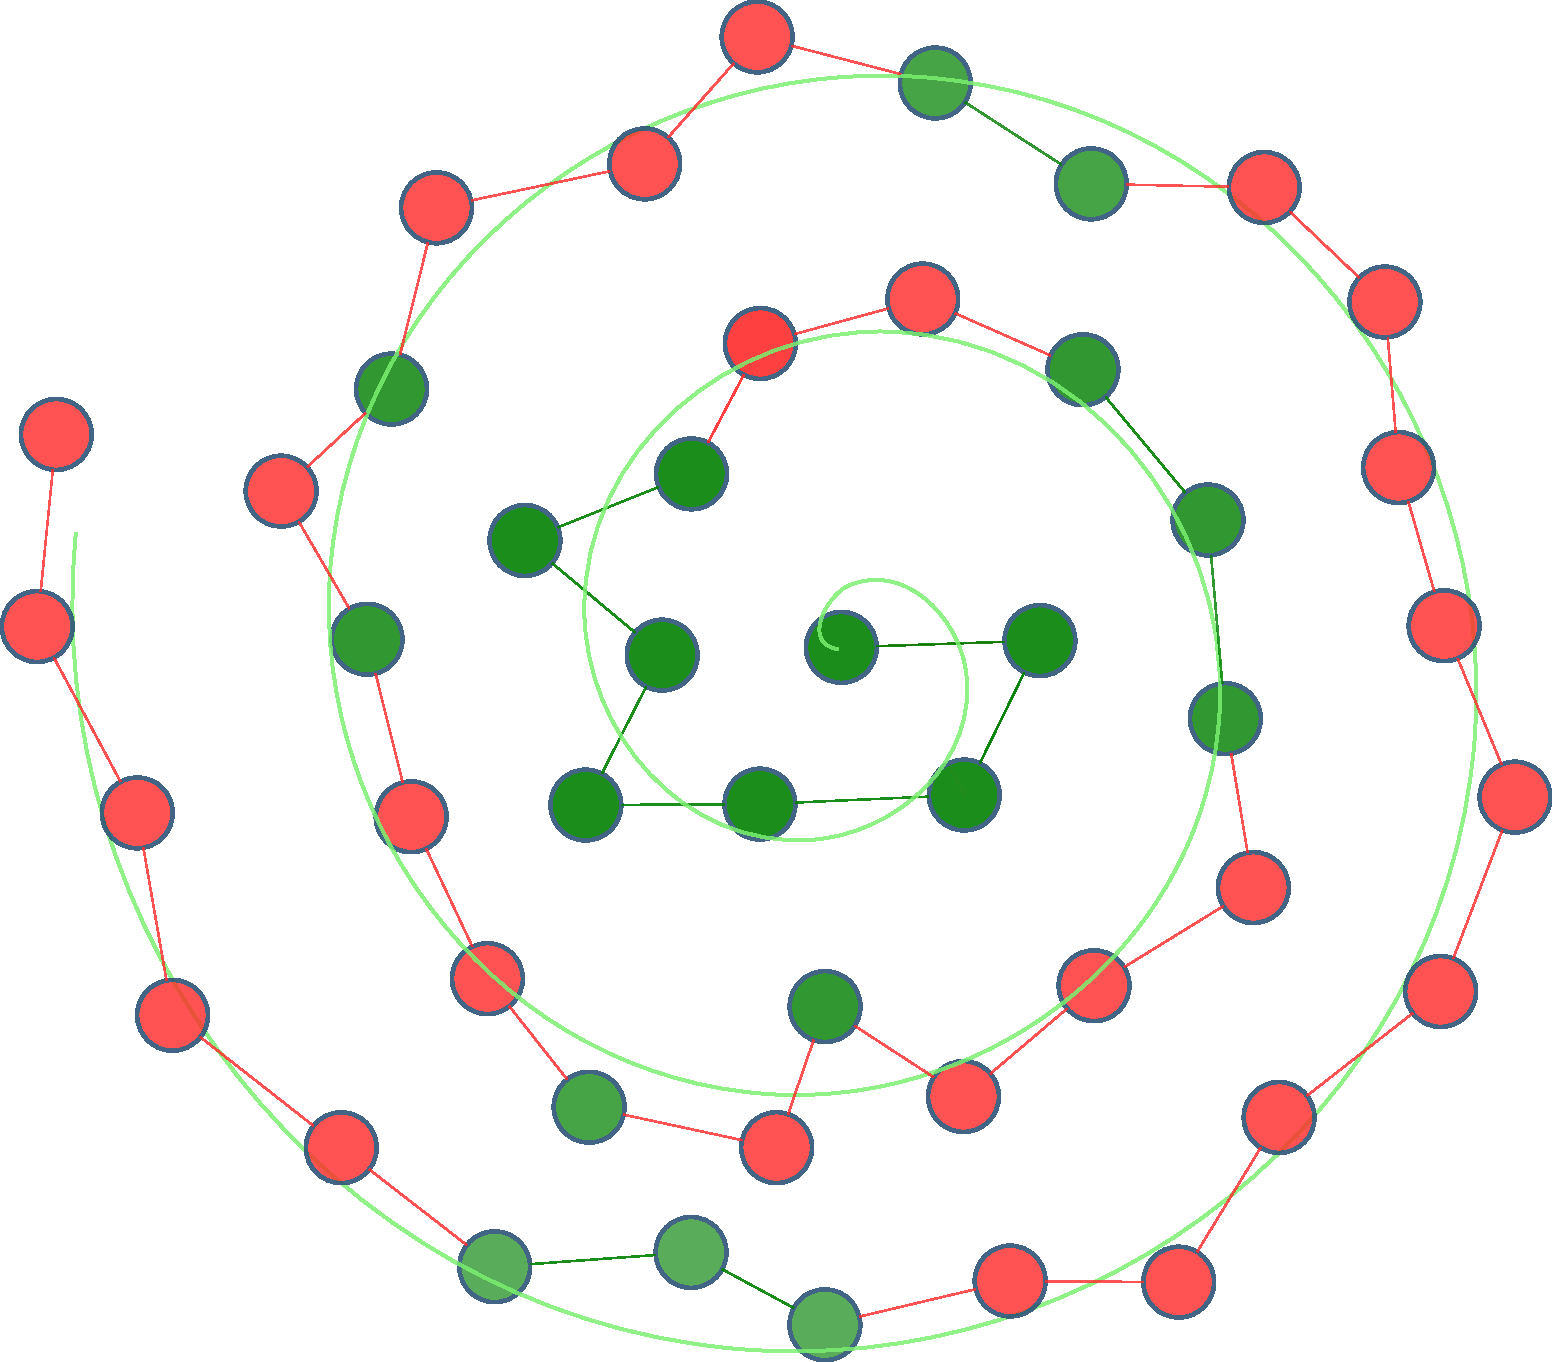
\includegraphics[width=45mm]{images/node_trajectory.pdf}}
		\caption{Learning procedure in a 2D visualisation}
		\label{fig:path_planning_on_graph}
	\end{figure}   

	\subsubsection{Real-Time Path Planning}

	This section defines the necessary terms to perform real-time path planning. Namely, it describes search, learning and execution.
	
	\begin{itemize}    
			 
		\item \textbf{Search:}
		The search consists of finding a path on the existing graphs that best represents the trajectory that the user is performing. This must be done while the demonstration is being recorded as shown in Fig.\ref{fig:trajectory}. The initial position of the paths is always known, which depends on the robot's last configuration, that is being manipulated and is a known configuration of nodes for all the $2n$ graphs. On the other hand, the target position is unknown. Throughout the demonstration for a time $t$, the goal is represented by a configuration of nodes at that precise time. At the end of the demonstration of length $T$, the path is smoothed, given that the goal is known. The execution consists of reproduce the smoothed path as an optimised set of nodes that are representative of the movement.
		
		\item \textbf{Learning:}
		The system must be able to learn during and after each demonstration. Lifelong learning is applied in a way that the graphs should extend their stored information while the demonstrator is performing an action. Namely if we consider a graph $G_j$ of a joint $j$ and a path $P_j$ of the same joint for a specific action $A$ that is being executed; it is possible to require a node that does not exist in the graph $G_j$, this node will be called $N_{candidate}$, and can be added to the graph under certain constraints as shown in the Fig. \ref{fig:path_planning_on_graph}. Where for each point that belongs to the demonstrated trajectory, the closest node in the graph is found as shown in \ref{fig:path_planning_on_graph}, subsequently the new nodes are added to complete the trajectory in Fig. \ref{fig:new_nodes_edges}, and finally the representative path is found in Fig. \ref{fig:node_trajectory}.
		
		On the other hand, as the number of trajectories increases, the libraries should increase in size and the path planning time should decrease, as shown in the results of \cite{Berenson2012, Coleman2015}. And finally, after learning, the path found can be reproduced in the robot at any point of time. 
		 
		\item \textbf{Constraints:}
		 In this section, the constraints necessary to perform path planning within the graph representation of the world are introduced.
		 
		 \begin{itemize}
		 	
		 	\item IsInside($p$, $j$): The Cartesian points $p$ found for all joints must be inside the workspace of the respective joint $j$. The robot's workspace is not the same workspace for each joint.
		 	\item IsNode($p$, $g_j$): The Cartesian point $p$ found for all joints is already a node in the graph $g_j$ if the corresponding joint is $j$. If it is not a node and it is inside the workspace, then find the nearest node. If the distance between the candidate node $N_{candidate}$ and the closest node $N_{closest}$ is smaller than the value of the fixed edge $d$ then $N_{closest}$ is added to the path and no new node is created.
		 	\item CreateNode($p$, $g_j$, $\Theta$, $occupied$): If the distance between $N_{candidate}$ and the closest node $N_{closest}$ is greater than $d$, then the candidate is added to the graph $g_j$ with the corresponding angular configuration of the angles to reach that position. The state ``occupied" is initialised with 1 or TRUE. This new node depends on the previous node where the joint was. For instance, there is a direct connection between these two nodes and the node $N_{candidate}$ is added also to the path.
		 	
		 \end{itemize} 
	\end{itemize} 

\section{Evaluation of the System}

	This section describes the evaluation of the framework in three sections. 
	
	\begin{itemize}
		
		\item The evaluation of the exploration phase of the framework is a comparison between the exploration time, the size of the graphs and the speed of path learning while performing a demonstration.
		
		\item The second evaluation corresponds to the path learning of the framework, namely a comparison of speed, accuracy of trajectories and smoothness of reproduction on real robots, such as QTrobot, Freddy and NAO.
		Also a comparison of these properties with other similar approaches such as $Lightning$ and $Thunder$. 
		
		\item The final evaluation is a user preference evaluation, where non-expert users are asked to perform a series of random upper body actions and evaluate the quality of the robot's reproduction, this can also be done in different robot platforms as mentioned before.
	
	\end{itemize}

\section{Project Plan}

	This section presents the project plan, which is divided into three sections: project packages, milestones and deliverables.

	\subsection{Work Packages}
	
	The work packages focus on the tasks necessary to complete each milestone, in this thesis the main focus is on implementing a framework for learning from demonstration on different robots.
	
	\subsubsection{The bare minimum will include the following package:}

		\begin{enumerate}
		    \item[WP1] Literature Study
		    \item[WP2] Pose estimation simulation for all robots
		    \item[WP3] Qtrobot environment learning by self-exploration
		    \item[WP4] Path planning framework development for QTrobot
		    \item[WP5] Trajectory learning from demonstration for QTrobot's library
		    \item[WP6] Experimentation and evaluation with QTrobot
		    \item[WP7] Freddy environment learning by self-exploration
		    \item[WP8] NAO environment learning by self-exploration
		    \item[WP9] Project Report
		\end{enumerate}
	
	\subsubsection{The expected project will include the following package:}
	
		\begin{enumerate}
			\item[WP10] Path planning framework development for Freddy
			\item[WP11] Trajectory learning from demonstration for Freddy's library
			\item[WP12] Experimentation and evaluation with Freddy
		\end{enumerate}
	
	\subsubsection{The desired project will include the following package:}
	
		\begin{enumerate}
			\item[WP13] Path planning framework development for NAO
			\item[WP14] Trajectory learning from demonstration for NAO's library
			\item[WP15] Experimentation and evaluation with NAO
			\item[WP16] Voice command integration for QTrobot 
		\end{enumerate}
	
	\subsection{Milestones}
		
		The milestones of the project are divided into tree main parts, the implementation of the framework itself for a base robot and then a generalisation to other platforms, as well as a comparison with similar approaches.
		
		\begin{enumerate}
		    \item[M1] Literature review completed and best practice identified
		  	\item[M2] Simulation of skeleton imitation by all robots, QTrobot, Kinova Gen3 a.k.a. Freddy and NAO through the transfer of human poses to the respective robot embodiments
		    \item[M3] Implementation of the framework, namely self-exploration and learning through demonstration
		    \item[M4] Evaluation of the approach and comparison with similar approaches on QTrobot, Freddy and NAO
		    \item[M5] Report submission
		\end{enumerate}
	
	\subsection{Project Schedule}

	\begin{figure}[h!]
	    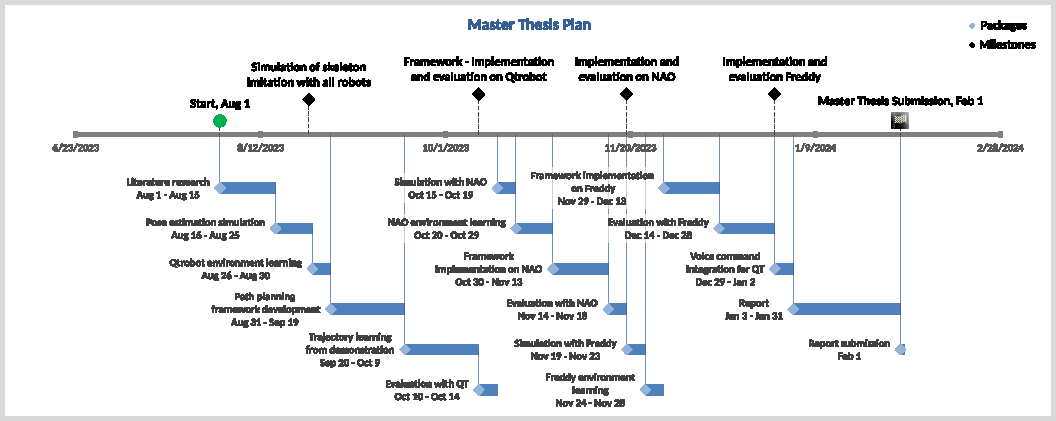
\includegraphics[width=\textwidth]{images/gantt.pdf}
	    \caption{Master thesis plan with milestones and packages}
	    \label{fig:gantt}
	\end{figure}

	\subsection{Deliverables}
	
	\subsubsection*{Minimum Viable}
	\begin{itemize}
	    \item This project aims to create a framework for real-time learning from demonstration and lifelong learning based on a graph representation of the environment, with the possibility of mapping static obstacles. The experiments will be performed by QTrobot and tested with real non-expert demonstrators. 
	\end{itemize}
	\subsubsection*{Expected}
	\begin{itemize}
	    \item The framework can be generalised and extended to the use of kinova arms a.k.a Freddy, due to the higher amount of DOF, to prove that the framework can be extended to any robot with two arms.
	\end{itemize}
	\subsubsection*{Desired}
	\begin{itemize}
		\item The framework can be generalised and extended to the use of NAO, due to the higher amount of DOF, to prove that the framework can be extended to any robot with two arms.
		
	    \item As the focus of this project is on a friendly system, it is desirable, but not necessary, to have at the top of the framework an interactive set of voice commands to start and stop the recordings, as well as to stop in case of emergency, this can be tested in QTrobot.
	\end{itemize}
	
	\nocite{*}
	
	\bibliographystyle{plainnat} % Use the plainnat bibliography style
	\bibliography{bibliography.bib} % Use the bibliography.bib file as the source of references
	
\end{document}
